\question 随着计算机技术的不断发展和对指令系统的合理性的研究,精简的指令系统(RISC)逐步取代CISC的重要位置。下面所述不是CISC的主要缺点的是
\par\twoch{20\%和80\%规律}{VLSI技术的不断发展引起的一系列问题}{\textcolor{red}{软硬件功能分配的问题}}{由于指令众多带来的编程困难}
\begin{solution}C。
CISC是既有简单指令又有复杂指令,后来世人发现典型程序中的80\%语句都是使用计算机中20\%的指令,而这20\%的指令都属于简单指令。所以,这个发现给予了研究人员一个警告,花再多的时间去研究复杂指令,也仅仅是有20\%的使用概率,这正是CISC的缺点。故A是CISC的主要缺点。
VLSI超大规模集成电路的技术发展与CISC的理念也造成冲突,CISC的指令执行速度较慢,不利于VLSI的实现(控制复杂)。故B是CISC的主要缺点。
CISC的指令系统复杂庞大,指令数目一般多达200\textasciitilde{}300条,也是CISC的主要缺点,也正是20\%与80\%规律的原因所在。故D是CISC的主要缺点。
而软硬件功能分配与指令系统没有直接关系,故C为干扰选项,本题选C。
\end{solution}
\question 下列对RISC的描述中正确的有 I.支持的寻址方式更多
II.大部分指令在一个机器周期完成 III.通用寄存器的数量多
IV.指令字长不固定
\par\twoch{I和IV}{\textcolor{red}{II和III}}{I、II和III}{I、II、III和IV}
\begin{solution}B。
I错误,RISC指令系统相对于CISC指令系统并没有产生出更多的寻址方式,相反,其寻址方式种类更少。
II正确,RISC指令是使用较多的简单指令条数去实现复杂的指令功能,绝大部分的指令是在一个机器周期完成的。
III正确,通用寄存器数量较多,可以提高指令的执行速度。
IV错误,RISC的指令长度固定。 综上,本题选B。
\end{solution}
\question 下列关于RISC的叙述中,错误的是( )
\par\fourch{\textcolor{red}{RISC普遍采用微程序控制器}}{RISC大多数指令在一个时钟周期内完成}{RISC的内部通用寄存器数量相对CISC多}{RISC的指令数、寻址方式和指令格式种类相对CISC少}
\begin{solution}应该记住RISC是和少、固定、小联系在一起的,但特殊的是,RISC的寄存器却多。
分析:由于RISC简单指令多,因此RISC大多数指令都在一个时钟周期内完成,故B正确;特殊的是,RISC的内部通用寄存器数量相对CISC多,故C正确;D选项体现了RISC的少,故D选项正确,最后得出正确答案为A。至于A选项,也可以联想一下,微程序不应该和简单的东西搭配在一起,后面会总结RISC控制器采用组合逻辑控制。RISC(Reduced
Instruction Set Computer)出现了。【总结】 CISC与RISC的区别见下表
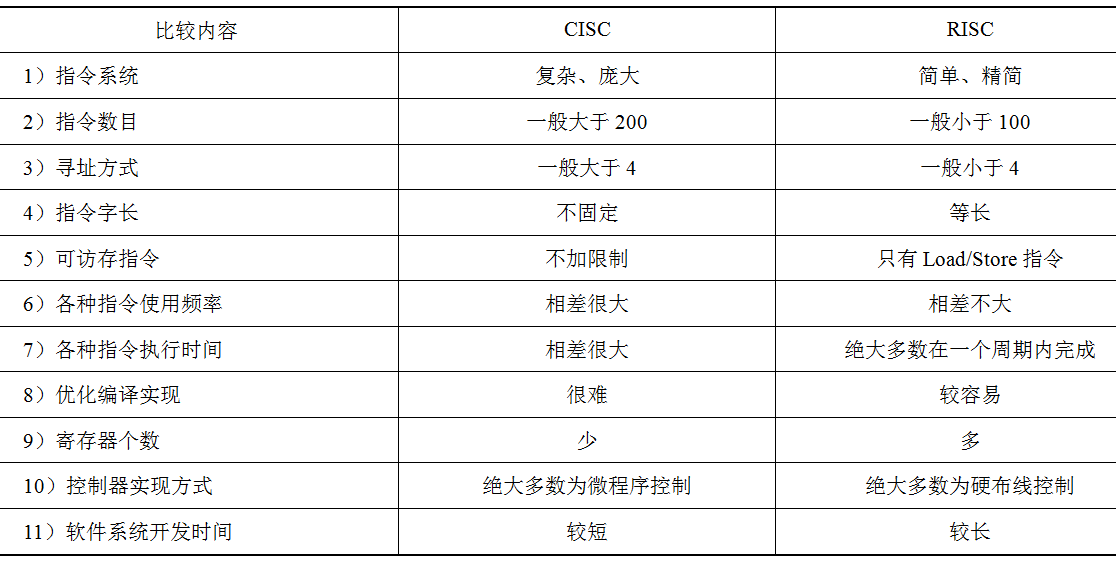
\includegraphics[width=3.46875in,height=1.73958in]{computerassets/8FD01177EADF3DDAF05DC032D8C42EE6.png}
\end{solution}
